% TODO:
%%%%%%%%%%%%%%%%%%%%%%%%%%%%%%%%%%%%%%%%%%%%%%%%%%%%%%%%%%%%%%%%%%%%%%%%%%
\chapter{Zobecněný hluboký zásobníkový automat a jeho redukce} \label{kap_pda_gen}

V~předchozí kapitole jsem se věnovala automatu se zjednodušeným zápisem pravidel. Toho jsem dosáhla tak, že jsem vymezila několik povolených typů.
Naskýtá se otázka, zda by nebylo výhodné zjednodušit přímo formu pravidla hlubokého zásobníkového automatu. Konkrétně by bylo možné vynechat hloubku expanze. Ta by tak nebyla definovaná v~pravidle, ale specifikovaná v~definici automatu. Tím bych dosáhla jistého zobecnění hlubokého zásobníkového automatu.

\section{Zobecněný hluboký zásobníkový automat}

Zobecněný hluboký zásobníkový automat (definice \ref{def_pda_gen}) vychází z~hlubokého zásobníkového automatu, ale s~hloubkou expanze pracuje jiným způsobem. Postupně prochází svým zásobníkem a aplikuje pravidlo typu $qA \rightarrow pv$ na nejvrchnější možný nevstupní symbol $A$. Dá se předpokládat, že tento model bude mít vyšší mocnost, neboť může expandovat symboly v~libovolné hloubce.

\begin{figure}[ht]
\centering
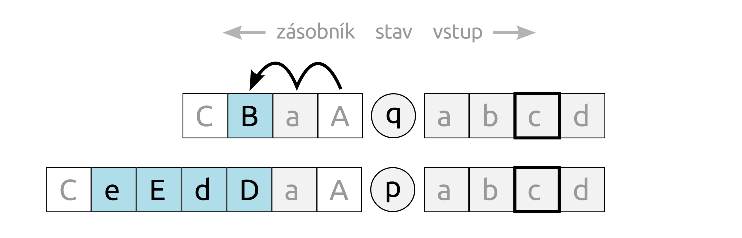
\includegraphics{img/bp_pda05.eps} \bigskip \\
\caption{Pravidlo $q B \rightarrow p DdEe$ lze ve zobecněném hlubokém zásobníkovém automatu v~aktuální konfiguraci aplikovat právě tehdy, když neexistuje pravidlo s~levou stranou $qA$.}
\end{figure}

\begin{Def} \label{def_pda_gen}
\emph{Zobecněný hluboký zásobníkový automat} je uspořádaná sedmice \\$M = (Q,\Sigma,\Gamma, R, s, S, F)$, 
kde $Q$, $\Sigma$, $\Gamma$, $s$, $S$, $F$ jsou definované stejně jako u~hlubokého zásobníkového automatu (definice \ref{def_deep_pda}) a $R$ je konečná množina pravidel typu 
\begin{equation*} 
(q, A, p, v) \in (Q \times (\Gamma-\Sigma) \times Q \times {\Gamma}^+)\textnormal{, píšeme }qA \rightarrow pv. 
\end{equation*}
Nechť $X$, $Y$ jsou dvě konfigurace $M$.  $M$ provede expanzi z~$X$ do $Y$, pokud $X = (q, w, uAz)$, $Y = (p, w, uvz)$, $qA \rightarrow pv \in R$, kde $p$, $q \in Q$, $w \in \Sigma^*$, $A \in \Gamma$, $u$, $v$, $z \in \Gamma^*$, a platí:
\begin{equation*} 
\{X \mid qX \rightarrow p'v' \in R\textnormal{, kde }X \in \mathrm{alph}(u) \cap (\Gamma - \Sigma)\textnormal{, }p' \in Q\textnormal{, }v' \in {\Gamma}^+ \} = \emptyset. 
\end{equation*}
\end{Def}

\begin{Def}\label{def_pda_gen_epsilon}
\emph{Zobecněný hluboký zásobníkový automat s~$\varepsilon$-pravidly} je zobecněný hluboký zásobníkový automat $M = (Q,\Sigma,\Gamma, R, s, S, F)$ rozšířený o~vymazávací pravidla typu\\ $qA \rightarrow p\varepsilon$, kde $p$, $q \in Q$, $A \in (\Gamma - \Sigma)$.
\end{Def}


%=========================================================================
 \section{Ekvivalence se stavovými gramatikami} \label{sec_ekv_state_grammars}

Když porovnám definici stavové gramatiky (\ref{def_state_gram}) s~definicí zobecněného hlubokého zásobníkového automatu (\ref{def_pda_gen}) je zřejmé, že se jedná o~ekvivalentní modely.

V~souvislosti s~kapitolou \ref{kap_teorie_hierarchie} lze o~tomto automatu prohlásit, že rodina jazyků, které přijímá, je identická s~rodinou kontextových jazyků. Dále z~definic \ref{def_state_gram_epsilon} a \ref{def_pda_gen_epsilon} vyplývá, že zobecněný hluboký zásobníkový automat s~$\varepsilon$-pravidly přijímá rodinu jazyků, která je identická s~rodinou  rekurzivně spočetných jazyků. Jinými slovy, tento automat má mocnost Turingova stroje.

%=========================================================================
\section{Omezení počtu nevstupních symbolů}

A. Meduna \cite{Meduna:StateGrammars} dokázal, že každá stavová gramatika s~$\varepsilon$-pravidly má svůj ekvivalentní protějšek se třemi nevstupními symboly. S~ohledem na výsledek kapitoly \ref{sec_ekv_state_grammars} je na místě prozkoumat, zda lze téhož dosáhnout i u~zobecněných hlubokých automatů.

V~algoritmu \ref{alg_gen_deep_pda_nonterm} demonstruji princip redukce nevstupních symbolů na symboly 0, 1 a \#. Hlavní myšlenka spočívá v~reprezentaci všech zásobníkových symbolů pomocí nul a jedniček. Symbol \# označuje fyzické dno zásobníku a umožňuje přesouvat symboly z~vrcholu na jeho konec. Zároveň k~symbolu \# zavádím binární ekvivalent, který označuje logické dno zásobníku. 

Princip simulace spočívá v~rozpoznání symbolu na vrcholu zásobníku pomocí pravidel z~množiny $R_{find}$ a jeho přesunu na dno zásobníku, případně expanzi pravidlem z~$R_{exp}$. Pokud dojde k~expanzi, aplikují se pravidla z~množiny $R_{move}$, která přesunou zbývající symboly na dno tak, aby se zásobník dostal do výchozího stavu pro další krok. Pokud pro žádný nevstupní symbol na~zásobníku expanze neproběhne, automat nahradí binární reprezentace vstupních symbolů původními symboly pomocí pravidel z~množiny $R_{end}$, smaže pomocné nevstupní symboly a přejde do koncového stavu.

\begin{Alg}\label{alg_gen_deep_pda_nonterm}
Převod zobecněného hlubokého zásobníkového automatu s~$\varepsilon$-pravidly na ekvivalentní se třemi nevstupními symboly.

\begin{list}{}{\setlength\parsep{0cm} \setlength\itemsep{0cm} \setlength\leftmargin{1em}}
   \item Vstup: $M = (Q,\Sigma,\Gamma, R, s, S, F)$ 
   \item Výstup: $M_{R} = (Q_{R}, \Sigma_{R}, {\Gamma}_{R}, R_{R}, s_{R},  S_{R}, F_{R})$ \medskip
  
   \item ${\Sigma}_{R} := \Sigma$
   \item ${\Gamma}_{R} := \Sigma \cup \{0,1,\#\}$
   \item $R_{R} := R_{find} \cup R_{next} \cup R_{exp} \cup R_{move} \cup R_{end}$
   \item $s_{R} := <start> $
   \item $S_{R} := \# $
   \item $F_{R} := \{<end>\} $ \medskip

\medskip

  \item Nechť $\Gamma = \{X_1, X_2, X_3, \dots, X_n\}$ pro $n \ge 1$ je množina všech zásobníkových symbolů v~$M$ a $X_0$ značí symbol $\#$. Pak definujme funkci $\varphi : \Gamma \cup \{\#\} \rightarrow \{0,1\}^*$ tak, že $\varphi (X_i)=0^i 1$ pro $i = 0,1,2,\dots,n$. \medskip

  \item Přidej do $Q_R$ pro každé $q \in Q$, $0 \le i \le n$ stavy:
  \item $<start>$, $<q, 0^i>$, $<q, 0^i 1>$, $<q, 0^i>'$, $<q, 0^i 1>'$, $<q, 0^i>''$, $<q, 0^i 1>''$, $<end>$.\medskip

  \item Pro každé $qA \rightarrow p B_0 B_1 \dots B_{j-1} B_{j} \in R$, kde $p, q \in Q$, $j \ge 0$, $B_0,B_1,\dots,B_j \in \Gamma$ a $A \in (\Gamma - \Sigma)$, 
          přidej $<q, \varphi (A)>$ do množiny $Q_{exp}$  a do $R_{exp}$ pravidla:

\begin{enumerate}
\renewcommand{\labelenumi}{(\roman{enumi})}

  \item $<start> \# \rightarrow <s, \varepsilon> \varphi(S)\varphi(\#)\#$,
  \item $<q, \varphi (A)> \# \rightarrow <p, \varepsilon>' \varphi(B_0)\varphi(B_1)\varphi(B_2) \dots \varphi(B_{j-1}) \varphi(B_{j}) \#$.

\suspend{enumerate}

  \item Pro každé $q \in Q$, $0 \le i < n$, $0 \le j \le n$ přidej do $R_{find}$ pravidla:

\resume{enumerate}
\renewcommand{\labelenumi}{(\roman{enumi})}

  \item $<q, 0^i> 0 \rightarrow <q, 0^{i+1}> \varepsilon $, $<q, 0^j> 1 \rightarrow <q, 0^j 1> \varepsilon $,
  \item $<q, 0^i>' 0 \rightarrow <q, 0^{i+1}>' \varepsilon $, $<q, 0^j>' 1 \rightarrow <q, 0^j 1>' \varepsilon $,
  \item $<q, 0^i>'' 0 \rightarrow <q, 0^{i+1}>'' \varepsilon $, $<q, 0^j>'' 1 \rightarrow <q, 0^j 1>'' \varepsilon $.

\suspend{enumerate}


  \item Přidej do $R_{next}$ pravidla:

\resume{enumerate}
\renewcommand{\labelenumi}{(\roman{enumi})}

  \item $<q, \varphi(X)> \# \rightarrow <q, \varepsilon> \varphi(X) \# $, kde $X \in \Gamma$, $q \in Q$, $<q, \varphi(X)> \notin Q_{exp}$,
  \item $<q, \varphi(\#) > \# \rightarrow <q, \varepsilon>'' \varphi(\#) \# $, kde $q \in Q$.

\suspend{enumerate}

  \item Přidej do $R_{move}$ pravidla:

\resume{enumerate}
\renewcommand{\labelenumi}{(\roman{enumi})}

  \item $<q, \varphi(X)>' \# \rightarrow <q, \varepsilon>' \varphi(X) \# $, kde $X \in \Gamma$, $q \in Q$,
  \item $<q, \varphi(\#) >' \# \rightarrow <q, \varepsilon> \varphi(\#) \# $, kde $q \in Q$.

\suspend{enumerate}

  \item Přidej do $R_{end}$ pravidla:

\resume{enumerate}
\renewcommand{\labelenumi}{(\roman{enumi})}

  \item $<q, \varphi(X) >'' \# \rightarrow <q, \varepsilon>'' X \# $, kde $X \in \Sigma$, $q \in Q$,
  \item $<q, \varphi(X) >'' \# \rightarrow <q, \varepsilon>'' \varphi(X) \# $, kde $X \in (\Gamma - \Sigma)$, $q \in Q$,
  \item $<q, \varphi(\#) >'' \# \rightarrow <end> \epsilon $, kde $q \in Q$.

\end{enumerate}

\end{list}
\end{Alg}

Z~uvedeného algoritmu vyplývá, že redukce neovlivní mocnost hlubokého zásobníkového automatu s~$\varepsilon$-pravidly. Pro automat bez $\varepsilon$-pravidel nelze tento postup použít. Zůstává tedy otázkou, zda je též zredukovatelný na tři nevstupní symboly.


%%%%%%%%%%%%%%%%%%%%%%%%%%%%%%%%%%%%%%%%%%%%%%%%%%%%%%%%%%%%%%%%%%%%%%%%%%%%%%%%%%%%%%%%%%%%%%%%%%%%%%%%%%%%%%%%%%%%%%%
\newpage

\begin{Example}\label{example_symbol}
$M$ je zobecněný hluboký zásobníkový automat a $M_{R}$ je jeho zredukovaná varianta se třemi nevstupními symboly zkonstruovaná podle algoritmu \ref{alg_gen_deep_pda_nonterm}. Nechť funkce $\varphi$ je definovaná jako :

\[ \varphi(x) = \left\{
  \begin{array}{l l}
    1 & \quad \text{pro $x = \#$}\\
    01 & \quad \text{pro $x = A$}\\
    001 & \quad \text{pro $x = B$}\\
    0001 & \quad \text{pro $x = C$}\\
    00001 & \quad \text{pro $x = D$}\\
    000001 & \quad \text{pro $x = d$}
  \end{array} \right.\]

\medskip

Následující definice automatů jsou jen částečné z~důvodu větší přehlednosti a pravidla jsou označena jednoznačným identifikátorem.
\bigskip

\setlength{\deftabcolsep}{\tabcolsep}
\setlength{\tabcolsep}{1pt}

\begin{tabular}{ll}

$M = ($&$\{s,p,q,r,\dots,f\},$ \\
     &$\{a,b,c,d,e\}, $\\
     &$\{a,b,c,d,e,A,B,C,D,E\},$ \\
     &$\{qB \rightarrow p Dd, \dots\},$\\
     &$s,$ \\
     &$S,$ \\
     &\{f\} )
\end{tabular}

\bigskip

\begin{tabular}{llp{12cm}l}

$M_{R} = ($ &$\{$ & $ <start>, <q, \varepsilon>,<q,1>,<q,0>,<q,01>,<q,00>,<q,001>, $\\ 
     && $ <p,\varepsilon>,<p,1>,<p,0>,<p,01>,<p,00>,<p,001>,<p,000> ,$\\ 
     && $ <p,0001>, <p,\varepsilon>',<p,1>',<p,0>',<p,01>',<p,00>', $\\ 
     && $ <p,001>',<p,000>',<p,0001>', \dots, <end>$\\ 
     &$\}$ \\
     &$\{$ & $a,b,c,d,e \ \}, $\\
     &$\{$ & $a,b,c,d,e, 0, 1, \# \},$ \\
     &$\{$ \\
     && 1 :\quad$ <q, \varepsilon> \ 0 \ \rightarrow \ <q, 0> \ \varepsilon ,$\\ 
     && 2 :\quad$ <q, 0> \ 1 \ \rightarrow \  <q, 01> \ \varepsilon ,$\\ 
     && 3 :\quad$ <q, 01> \ \# \ \rightarrow \ <q, \varepsilon> \ 01\# ,$\\ 
     && 4 :\quad$ <q, \varepsilon> \ 0 \ \rightarrow \  <q, 0> \ \varepsilon ,$\\ 
     && 5 :\quad$ <q, 0> \ 0 \ \rightarrow \ <q, 00> \ \varepsilon ,$\\ 
     && 6 :\quad$ <q, 00> \  0  \ \rightarrow \ <q, 001> \ \varepsilon ,$\\ 
     && 7 :\quad$ <q, 001> \  \# \ \rightarrow \ <p,\varepsilon>' \ 00001000001\# ,$\\ 
     && 8 :\quad$ <p,\varepsilon>' \ 0 \ \rightarrow \  <p,0>' \ \varepsilon ,$\\ 
     && 9 :\quad$ <p,0>' \  0 \ \rightarrow \  <p,00>' \ \ \varepsilon ,$\\ 
     && 10:\quad$ <p,00>' \ 0 \ \rightarrow \   <p,000>' \ \varepsilon ,$\\ 
     && 11:\quad$ <p,000>' \  1 \ \rightarrow \ <p,0001>' \ \varepsilon ,$\\ 
     && 12:\quad$ <p,0001>' \ \# \ \rightarrow <p,\varepsilon>' \ 0001\# ,$\\ 
     && 13:\quad$ <p,\varepsilon>' \  1 \ \rightarrow \ <p,1>' \ \varepsilon ,$\\ 
     && 14:\quad$ <p,1>' \ \# \ \rightarrow \ <p,\varepsilon> \ 1\# ,$\\ 
     && \dots\\ 
     & $ \},$ \\
     &\multicolumn{2}{l}{$<start>,$} \\
     &\multicolumn{2}{l}{$\#,$} \\
     &$\{$&${<end>}\ \}$ )
\end{tabular}
\bigskip

\setlength{\tabcolsep}{\deftabcolsep}

\newpage
Ukázka aplikace pravidla $qB \rightarrow p Dd$ v~konfiguraci $(q, abc, ABC)$ v~zobecněném hlubokém zásobníkovém automatu zkonstruovaném podle algoritmu \ref{alg_gen_deep_pda_nonterm}.
\medskip

\begin{tabular}{lllll|l|l}
                & $( <q, \varepsilon>$,  & $abc$, & $0100100011\#$         $)$ && $ABC\#$ \\
$\Rightarrow$   & $( <q, \mathbf{0}>$,   & $abc$, & $100100011\#$         $)$ &[1]& \\
$\Rightarrow$   & $( <q, 0\mathbf{1}>$,  & $abc$, & $00100011\#$         $)$ &[2]&   $BC\#$ & přečteno A~\\
$\Rightarrow$   & $( <q, \varepsilon>$,  & $abc$, & $00100011\mathbf{01}\#$         $)$ &[3]& $BC\#\mathbf{A}$ & přesun A~\\
$\Rightarrow$   & $( <q, \mathbf{0}>$,   & $abc$, & $010001101\#$         $)$ &[4]& \\
$\Rightarrow$   & $( <q, 0\mathbf{0}>$,  & $abc$, & $10001101\#$         $)$ &[5]& \\
$\Rightarrow$   & $( <q, 00\mathbf{1}>$, & $abc$, & $0001101\#$         $)$ &[6]&    $C\#A$ & přečteno B \\
$\Rightarrow$   & $( <p,\varepsilon>'$,  & $abc$, & $0001101\mathbf{00001000001}\#$         $)$ &[7]& $C\#A\mathbf{Dd}$ & expanze B \\
$\Rightarrow$   & $( <p,\mathbf{0}>'$,   & $abc$, & $00110100001000001\#$         $)$ &[8]& \\
$\Rightarrow$   & $( <p,0\mathbf{0}>'$,  & $abc$, & $0110100001000001\#$         $)$ &[9]& \\
$\Rightarrow$   & $( <p,00\mathbf{0}>'$, & $abc$, & $110100001000001\#$         $)$ &[10]& \\
$\Rightarrow$   & $( <p,000\mathbf{1}>'$,& $abc$, & $10100001000001\#$         $)$ &[11]& $\#ADd$ & přečteno C  \\
$\Rightarrow$   & $( <p,\varepsilon>'$,  & $abc$, & $10100001000001\mathbf{0001}\#$         $)$ &[12]& $\#ADd\mathbf{C}$ & přesun C \\
$\Rightarrow$   & $( <p,\mathbf{1}>'$,   & $abc$, & $01000010000010001\#$         $)$ &[13]& $ADdC$ & dno zásobníku \\
$\Rightarrow$   & $( <p,\varepsilon>$,   & $abc$, & $01000010000010001\mathbf{1}\#$         $)$ &[14]& $ADdC\mathbf{\#}$ & konec
\end{tabular}

\end{Example}
%%%%%%%%%%%%%%%%%%%%%%%%%%%%%%%%%%%%%%%%%%%%%%%%%%%%%%%%%%%%%%%%%%%%%%%%%%%%%%%%%%%%%%%%%%%%%%%%%%%%%%%%%%%%%%%%%%%%%%%
%=========================================================================
\section{Omezení počtu stavů}

Pro každou stavovou gramatiku s~$\varepsilon$-pravidly dle A. Meduny \cite{Meduna:StateGrammars} platí, že existuje ekvivalentní stavová gramatika s~právě třemi stavy. V~algoritmu \ref{alg_gen_deep_pda_state} ukazuji, že totéž platí pro zobecněné hluboké zásobníkové automaty.

Pokud automat může být jen v~jednom ze tří stavů, je zřejmé, že informace o~stavu simulovaného automatu musí být součástí každého nevstupního symbolu. Musela jsem tedy najít způsob, jak přepsat stavy ve všech nevstupních symbolech na aktuální hodnotu. 

Zvolila jsem princip \uv{kruhového přepisování}. Pokud nad množinou stavů definuji uspořádání, pak mohu přepsat první stav na druhý, druhý na třetí, \dots, předposlední na poslední a poslední na první. Po konečném počtu kroků jsem schopna získat libovolný stav bez ohledu na jeho pořadí. Počet těchto kroků určuje symbol čítače, jehož hodnota se po každé změně stavu ve všech nevstupních symbolech sníží o~jedna. 

Zobecněný hluboký zásobníkový automat expanduje nejvrchnější nevstupní symbol, pro který je to možné. Proto ke každému nevstupnímu symbolu s~upravených stavem přidávám apostrof. Pro takový symbol v~daném stavu neexistuje pravidlo a automat se přesune na další symbol až po konec zásobníku. Po snížení hodnoty čítače se ze symbolů na zásobníku odstraní apostrofy a v~případě, že je čítač vynulovaný, se provede expanze. Pokud expanze způsobí změnu stavu, vygeneruje se nový čítač a celý postup se opakuje.

Funkčnost tohoto principu je závislá na rozdělení pravidel mezi tři stavy tak, aby automat v~žádném případě nemohl vykonat nežádaný krok. V~algoritmu \ref{alg_gen_deep_pda_state} řeším tento problém následovně. Množina $R_{\alpha}$ obsahuje pravidla pro expanzi, změnu hodnoty čítače a nastavení příznaku expanze. Pravidla z~$R_{\beta}$ mění stav v~nevstupních symbolech a symboly značí apostrofem. Množina pravidel $R_{\gamma}$ odstraňuje apostrofy z~nevstupních symbolů a podle příznaku na konci zásobníku automat přejde do stavu pro expanzi nebo pro aktualizaci stavů.

\begin{Alg}\label{alg_gen_deep_pda_state}
Převod zobecněného hlubokého zásobníkového automatu s~$\varepsilon$-pravidly na ekvivalentní s~redukcí na tři stavy.

\begin{list}{}{\setlength\parsep{0cm} \setlength\itemsep{0cm} \setlength\leftmargin{1em}}
   \item Vstup: $M = (Q,\Sigma,\Gamma, R, s, S, F)$ 
   \item Výstup: $M_{R} = (Q_{R}, \Sigma_{R}, {\Gamma}_{R}, R_{R}, s_{R},  S_{R}, F_{R})$ \medskip

   \item ${\Sigma}_{R} := \Sigma$
   \item ${\Gamma}_{R} := \Sigma \cup {\Gamma}_{R}'$
   \item $Q_{R} := \{s_\alpha, s_\beta, s_\gamma \}$
   \item $R_{R} := R_{\alpha} \cup R_{\beta} \cup R_{\gamma}$
   \item $s_{R} := s_{\alpha} $
   \item $S_{R} := <start> $
   \item $F_{R} := \{s_{\alpha}\} $ \medskip

   \item Nechť $Q = \{s_0, s_1, s_2, \dots,s_{|Q-1|}\}$, kde $s_0 = s$ je počáteční stav v~$M$. Nechť $s_{|Q|} = s_0$.\medskip

   \item Pro každé $q \in Q$, $X \in (\Gamma - \Sigma)$, $j \in \{1,2,3,\dots,|Q|\}$ přidej do ${\Gamma}_{R}'$ symboly :
   \item $<start>, <j>, <q, X>, <q, X>', <q, \#>, <q, \#>_{set}, <q, \#>_{exp}$.\medskip

   \item Pro každé $qA \rightarrow p b_0 B_1 b_1 B_2 b_2 \dots b_{j-1} B_{j} b_j \in R$, kde $p, q \in Q$, $j \ge 0$, $b_0,b_1,\dots,b_j \in {\Sigma}^*$ a $A, B_1,B_2,\dots,B_j \in (\Gamma - \Sigma)$. 
         Nechť $p=s_x$ a $q=s_y$, kde $x$, $y$ jsou indexy stavů $p$, $q$, pak označme $k = (x - y) \textrm{ \% } |Q|$ . 
         Přidej do $R_\alpha$ pravidla:

\begin{enumerate}
\renewcommand{\labelenumi}{(\roman{enumi})}

   \item $s_\alpha <start> \rightarrow s_\alpha <s_0, S> <s_0, \#>$,
   \item  $s_\alpha <q, A> \rightarrow s_\alpha b_0 <q, B_1> b_1 <q, B_2> b_2 \dots b_{j-1} <q, B_j> b_j$ pokud $p = q$,
   \item  $s_\alpha <q, A> \rightarrow s_\beta <k> b_0 <q, B_1> b_1 <q, B_2> b_2 \dots b_{j-1} <q, B_j> b_j$ pro $p \ne q$. 

\suspend{enumerate}

   \item Přidej do $R_\beta$ pravidla:

\resume{enumerate}
\renewcommand{\labelenumi}{(\roman{enumi})}

   \item $s_\beta <s_i, X> \rightarrow s_\beta <s_{i+1}, X>'$ pro každé $s_i \in Q$ a každé $X \in (\Gamma - \Sigma)$,
   \item $s_\beta <s_i, \#> \rightarrow s_\alpha <s_{i+1}, \#>_{set}$ pro každé $s_i \in Q$.

\suspend{enumerate}

   \item Přidej do $R_\alpha$ pravidla:

\resume{enumerate}{\setlength\leftmargin{1em}}
\renewcommand{\labelenumi}{(\roman{enumi})}

   \item $s_\alpha <j> \rightarrow s_\gamma <j - 1 > $ pro každé $j \in \{2,3,\dots,|Q|\}$,
   \item $s_\alpha <1> \rightarrow s_\alpha \varepsilon $,
   \item $s_\alpha <s_i, \#>_{set} \rightarrow s_\gamma <s_{i}, \#>_{exp}$ pro každé $s_i \in Q$,
   \item $s_\alpha <q, \#> \rightarrow s_\alpha \varepsilon $ pro každé $q \in F$.

\suspend{enumerate}{\setlength\leftmargin{1em}}

   \item Přidej do množiny $R_\gamma$ pravidla:

\resume{enumerate}
\renewcommand{\labelenumi}{(\roman{enumi})}

   \item $s_\gamma <s_i, X>' \rightarrow s_\gamma <s_i, X> $ pro každé $s_i \in Q$ a každé $X \in (\Gamma - \Sigma)$,
   \item $s_\gamma <s_i, \#>_{set} \rightarrow s_\beta <s_i, \#>$ pro každé $s_i \in Q$,
   \item $s_\gamma <s_i, \#>_{exp} \rightarrow s_\alpha <s_{i}, \#>$ pro každé $s_i \in Q$.

\end{enumerate}

\end{list}
\end{Alg}

Každý zobecněný hluboký zásobníkový automat s~$\varepsilon$-pravidly lze převést na ekvivalentní se třemi stavy, jak vyplývá z~algoritmu \ref{alg_gen_deep_pda_state}. Otázka, zda lze stejně zredukovat automat bez $\varepsilon$-pravidel, zůstává otevřená.

%%%%%%%%%%%%%%%%%%%%%%%%%%%%%%%%%%%%%%%%%%%%%%%%%%%%%%%%%%%%%%%%%%%%%%%%%%%%%%%%%%%%%%%%%%%%%%%%%%%%%%%%%%%%%%%%%%%%%%%

\newpage
\begin{Example}\label{example_state}
$M$ je zobecněný hluboký zásobníkový automat a $M_{R}$ je jeho zredukovaná varianta zkonstruovaná podle algoritmu \ref{alg_gen_deep_pda_state}. Definice automatů jsou pro větší přehlednost neúplné. Na pravidla se odkazuji pomocí identifikátorů.
\bigskip

\setlength{\deftabcolsep}{\tabcolsep}
\setlength{\tabcolsep}{1pt}

\begin{tabular}{ll}

$M = ($&$\{s,p,q,r,\dots,f\},$ \\
     &$\{a,b,c,d,e\}, $\\
     &$\{a,b,c,d,e,A,B,C,D,E\},$ \\
     &$\{pB \rightarrow r Dd, \dots\},$\\
     &$s,$ \\
     &$S,$ \\
     &\{f\} )
\end{tabular}

\bigskip



\begin{tabular}{llp{12cm}l}

$M_{R} = ($ &$\{$ & $s_{\alpha}, s_{\beta},s_{\gamma} \ \}, $\\
     &$\{$ & $a,b,c,d,e \ \}, $\\
     &$\{$ & $a,b,c,d,e, <start>, <1>, <2>, \dots, <p, A>, <p, B>, <p, C>, $\\
     &&$  <p, D>,<p, A>',<p, B>',<p, C>', <p, D>', <q, A>, <q, B>, $\\
     &&$ <q, C>, <q, D>,<q, A>',<q, B>',<q, C>', <q, D>',<r, A>, $\\
     &&$ <r, B>, <r, C>, <r, D>,<r, A>',<r, B>',<r, C>', <r, D>',$\\
     &&$ <p, \#>, <p, \#>_{set}, <p, \#>_{exp}, <q, \#>, <q, \#>_{set}, <q, \#>_{exp}, $\\
     &&$ <r, \#>, <r, \#>_{set}, <r, \#>_{exp}, \dots$\\
     & $ \},$ \\
     &$\{$ \\
     && 1 :\quad$ s_{\alpha} \ <p,B>\ \rightarrow \ s_{\beta} <2>\ <p,D>\ d  ,$\\ 
     && 2 :\quad$ s_{\beta}\ <q,A>\ \rightarrow\ s_{\beta}\ <q,A>'  ,$\\ 
     && 3 :\quad$ s_{\beta}\ <q,D>\ \rightarrow\ s_{\beta}\ <q,D>'   ,$\\ 
     && 4 :\quad$ s_{\beta}\ <p,\#>\ \rightarrow\ s_{\alpha}\ <q,\#>_{set}  ,$\\ 
     && 5 :\quad$ s_{\alpha}\ <2>\ \rightarrow\ s_{\gamma}\ <1>  ,$\\ 
     && 6 :\quad$ s_{\gamma}\ <q,A>'\ \rightarrow\ s_{\gamma}\ <q,A>  ,$\\ 
     && 7 :\quad$ s_{\gamma}\ <q,D>'\ \rightarrow \ s_{\gamma}\ <q,D>  ,$\\ 
     && 8 :\quad$ s_{\gamma}\ <q, \#>_{set}\ \rightarrow\ s_{\beta}\ <q, \#>  ,$\\ 
     && 9 :\quad$ s_{\beta}\ <r,A>\ \rightarrow\ s_{\beta}\ <r,A>'  ,$\\ 
     && 10:\quad$ s_{\beta}\ <r,D>\ \rightarrow\ s_{\beta}\ <r,D>'  ,$\\ 
     && 11:\quad$ s_{\beta}\ <r,\#>\ \rightarrow\ s_{\alpha}\ <r,\#>_{set}  ,$\\ 
     && 12:\quad$ s_{\alpha}\ <1>\  \rightarrow\ s_{\alpha}\ \varepsilon  ,$\\ 
     && 13:\quad$ s_{\alpha}\ <r,\#>_{set}\ \rightarrow\ s_{\gamma}\ <r, \#>_{exp}  ,$\\ 
     && 14:\quad$ s_{\gamma}\ <r,A>'\ \rightarrow\ s_{\gamma}\ <r,A>  ,$\\ 
     && 15:\quad$ s_{\gamma}\ <r,D>'\ \rightarrow\ s_{\gamma}\ <r,D>  ,$\\ 
     && 16:\quad$ s_{\gamma}\ <r, \#>_{exp}\ \rightarrow\ s_{\alpha}\ <r, \#>  ,$\\ 
     &&$ \dots$ \\
     & $ \},$ \\
     &\multicolumn{2}{l}{$s_{\alpha},$} \\
     &\multicolumn{2}{l}{$<start>,$} \\
     &$\{$&$s_{\alpha}\ \}$ )
\end{tabular}
\bigskip



\setlength{\tabcolsep}{\deftabcolsep}

\newpage
Ukázka simulace pravidla $pB \rightarrow r Dd$ v~konfiguraci $(p, abc, ABc)$ v~zobecněném hlubokém zásobníkovém automatu $M_{R}$ zkonstruovaném z~automatu $M$ podle algoritmu \ref{alg_gen_deep_pda_state}.\medskip


\setlength{\deftabcolsep}{\tabcolsep}
\setlength{\tabcolsep}{4pt}

\begin{tabular}{llllc|l}
                & $( s_{\alpha}$,  & $abc$, & $<p,A> <p,B> c <p, \#>$         $)$ & &  \\
$\Rightarrow$   & $( \mathbf{s_{\beta}}$,   & $abc$, & $<p,A> \mathbf{<2> <p,D> d} c <p, \#>$   $)$ & [1] \quad&\quad expanze $pB \rightarrow r Dd$ \\
$\Rightarrow$   & $( s_{\beta}$,   & $abc$, & $\mathbf{<q,A>'} <2> <p,D> d c <p, \#>$         $)$  & [2] \quad&\quad přepis stavů $q$ na $p$\\
$\Rightarrow$   & $( s_{\beta}$,   & $abc$, & $<q,A>' <2> \mathbf{<q,D>'} d c <p, \#>$         $)$  & [3] \quad&\quad \\
$\Rightarrow$   & $( \mathbf{s_{\alpha}}$,   & $abc$, & $<q,A>' <2> <q,D>' d c \mathbf{<q, \#>_{set}}$         $)$  & [4] \quad&\quad nastavení příznaku $set$\\
$\Rightarrow$   & $( \mathbf{s_{\gamma}}$,  & $abc$, & $<q,A>' \mathbf{<1>} <q,D>' d c <q, \#>_{set}$  $)$  & [5] \quad&\quad snížení hodnoty čítače \\
$\Rightarrow$   & $( s_{\gamma}$,  & $abc$, & $\mathbf{<q,A>} <1> <q,D>' d c <q, \#>_{set}$  $)$  & [6] \quad&\quad odznačení symbolů \\
$\Rightarrow$   & $( s_{\gamma}$,  & $abc$, & $<q,A> <1> \mathbf{<q,D>} d c <q, \#>_{set}$  $)$  & [7] \quad&\quad  \\
$\Rightarrow$   & $( \mathbf{s_{\beta}}$,  & $abc$, & $<q,A> <1> <q,D> d c \mathbf{<q, \#>}$  $)$  & [8] \quad&\quad  odstranění příznaku $set$\\
$\Rightarrow$   & $( s_{\beta}$,  & $abc$, & $\mathbf{<r,A>'} <1> <q,D> d c <q, \#>$  $)$  & [9] \quad&\quad  přepis stavů $p$ na $r$\\
$\Rightarrow$   & $( s_{\beta}$,  & $abc$, & $<r,A>' <1> \mathbf{<r,D>'} d c <q, \#>$  $)$  & [10] \quad&\quad  \\
$\Rightarrow$   & $( \mathbf{s_{\alpha}}$,  & $abc$, & $<r,A>' <1> <r,D>' d c \mathbf{<r, \#>_{set}}$  $)$  & [11] \quad&\quad  nastavení příznaku $set$\\
$\Rightarrow$   & $( s_{\alpha}$,  & $abc$, & $<r,A>' <r,D>' d c <r, \#>_{set}$  $)$  & [12] \quad&\quad  vynulování čítače\\
$\Rightarrow$   & $( \mathbf{s_{\gamma}}$,  & $abc$, & $<r,A>' <r,D>' d c \mathbf{<r, \#>_{exp}}$  $)$  & [13] \quad&\quad  nastavení příznaku $exp$\\
$\Rightarrow$   & $( s_{\gamma}$,  & $abc$, & $\mathbf{<r,A>} <r,D>' d c <r, \#>_{exp}$  $)$  & [14] \quad&\quad  odznačení symbolů\\
$\Rightarrow$   & $( s_{\gamma}$,  & $abc$, & $<r,A> \mathbf{<r,D>} d c <r, \#>_{exp}$  $)$  & [15] \quad&\quad  \\
$\Rightarrow$   & $( \mathbf{s_{\alpha}}$,  & $abc$, & $<r,A> <r,D> d c \mathbf{<r, \#>}$  $)$  & [16] \quad&\quad  konec

\end{tabular}

\setlength{\tabcolsep}{\deftabcolsep}

\end{Example}


%%%%%%%%%%%%%%%%%%%%%%%%%%%%%%%%%%%%%%%%%%%%%%%%%%%%%%%%%%%%%%%%%%%%%%%%%%%%%%%%%%%%%%%%%%%%%%%%%%%%%%%%%%%%%%%%%%%%%%%

%=========================================================================
